\documentclass[a4paper]{article}
\usepackage[T1]{fontenc}
\usepackage[utf8]{inputenc}
\usepackage[finnish]{babel}
\usepackage{graphicx}
\title{Tietokantasovellus-harjoitustyön dokumentaatio}
\author{Miika Hänninen}
\begin{document}
\maketitle
\tableofcontents
\section{Johdanto}
Tämän tietokantasovellus-harjoitustyön aiheena on drinkkiarkisto. Drinkkiarkiston tarkoitus on olla jokaisen kotibaarimestarin apuväline jolla löytää uudenlaisia juomia kokeiltavaksi, sekä palauttaa tuttujen drinkkien reseptit mieleen. Arkistosta kuka tahansa pystyy etsimään juomia esimerkiksi nimen, juomatyypin tai ainesosien perusteella. Kirjautuneet käyttäjät voivat luoda drinkkireseptejä ehdotuksiksi, jotka eivät näy suurelle yleisölle ennen kuin ylläpitäjä on ne hyväksynyt.

Projekti toteutetaan javascriptillä käyttäen alustana nodejs:ää. Tietokantana toimii PostgreSQL. Web-frameworkina toimii express. Dokumentaatio kirjoitetaan latexilla. Sovellus ei vaadi käyttäjän selaimelta javascript-tukea. Sovelluksen kehittämisen helpottamiseksi projektille on vagrant-konfiguraatio. Vagrant luo virtuaalikoneen joka vastaa mahdollisimman paljon tuotantoympäristöä ja sisältää kaiken tarpeellisen sovelluksen ajamiseen. 

Valmis ohjelmisto ajetaan herokussa. Jatkuvan integroinnin palvelu Travis kääntää uuden version ohjelmistosta aina kun githubiin pushataan uusi versio lähdekoodista, ja siirtää sen suoraan herokuun.
\pagebreak
\section{Yleiskuva järjestelmästä}
\subsection{Käyttötapauskaavio}
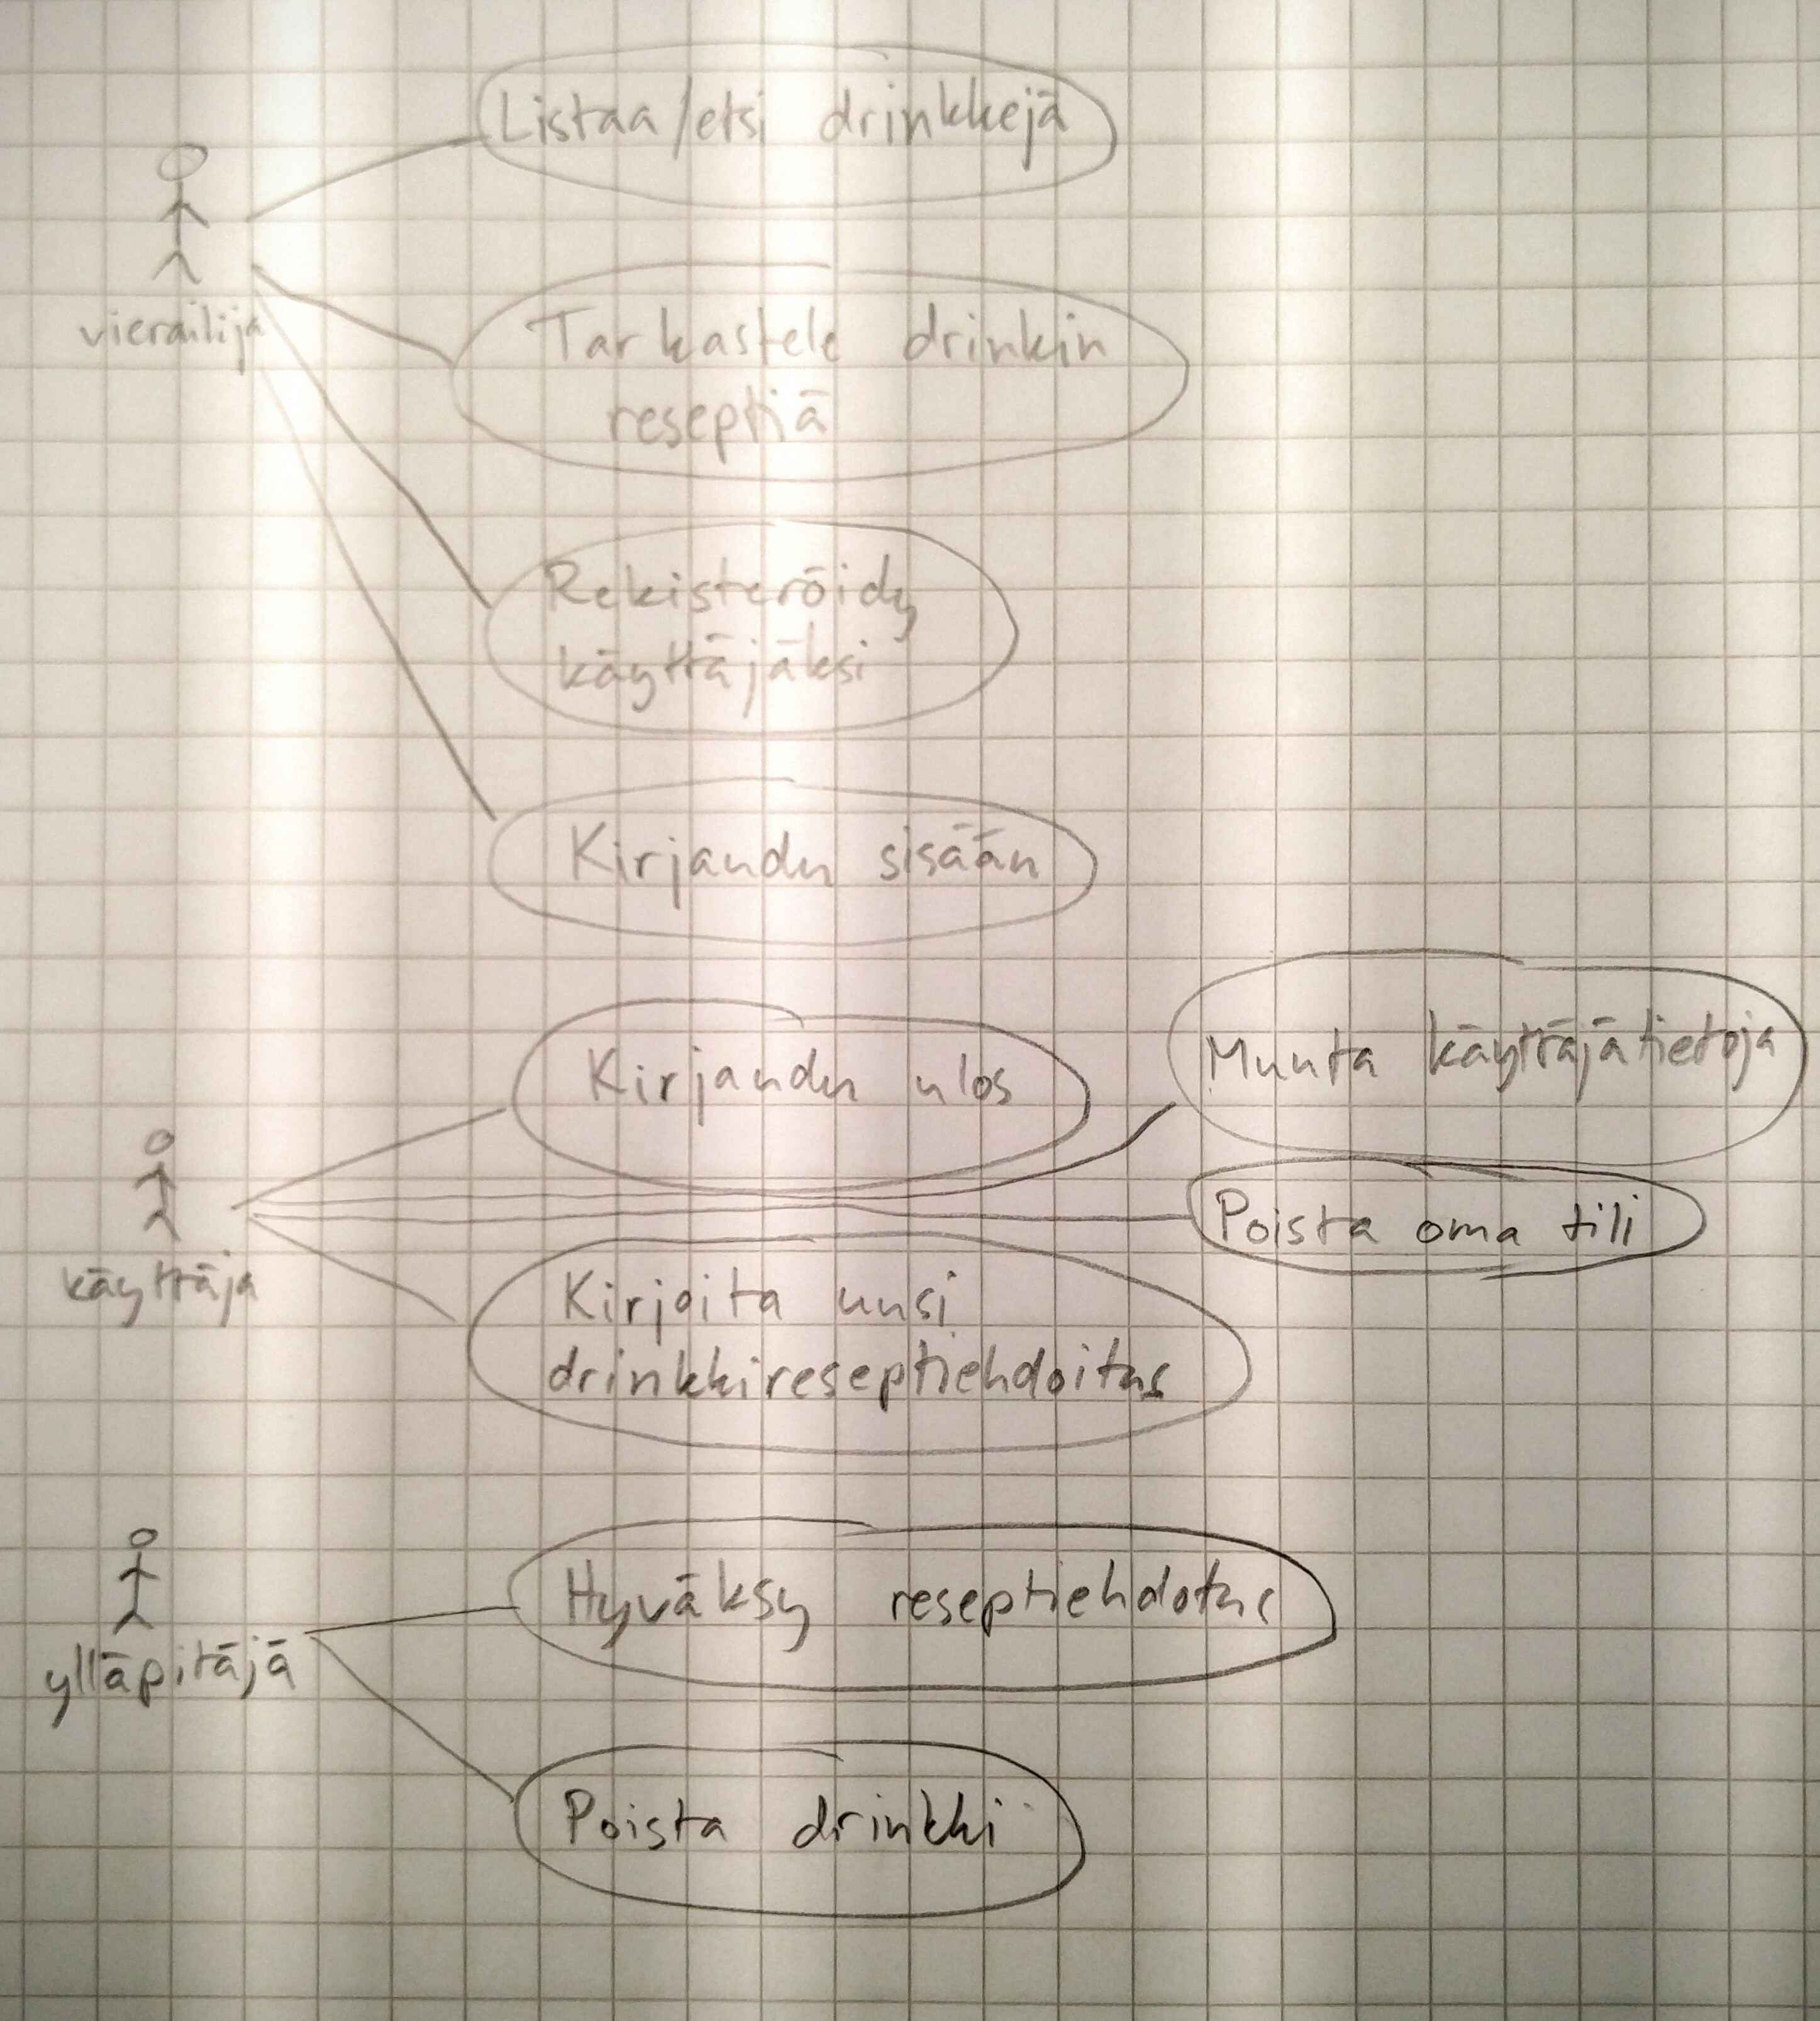
\includegraphics[width=\textwidth]{usecase-diagram}
\subsection{Käyttäjäryhmät}
Vierailija
\begin{quote}
  Vierailijalla tarkoitetaan ketä tahansa joka vierailee sivulla.
\end{quote}
Käyttäjä
\begin{quote}
  Käyttäjä on sivustolle rekisteröitynyt ja sisäänkirjautunut vierailija.
\end{quote}
Ylläpitäjä
\begin{quote}
  Ylläpitäjä on käyttäjä, jonka tehtäviin ja oikeuksiin kuuluu reseptien hallinnointi.
\end{quote}

\subsection{Käyttötapauskuvaukset}
\end{document}
